\usepackage{listings}
\usepackage{mfirstuc}
\usepackage{xstring}
\newcommand{\iH}{\ptp[h]\xspace}
\newcommand{\iK}{\ptp[k]\xspace}
\newcommand{\iI}{\ptp[i]\xspace}
\newcommand{\iJ}{\ptp[j]\xspace}

\newcommand{\sset}{\mathcal{S}}


%%%%%%%%%%%%%%%%%%%%%%%%%%%%%%%%%%%%%%%%%%%%%%%%%%%%%%%%%%%%%%%%%%%%%%%%%%%%%
%%%                            ChorGrapm macros                           %%%
%%%%%%%%%%%%%%%%%%%%%%%%%%%%%%%%%%%%%%%%%%%%%%%%%%%%%%%%%%%%%%%%%%%%%%%%%%%%%

\newif\ifcp
\cpfalse
\newcommand{\gname}[1][i]{\ifcp{\colorNode{\scriptstyle\textsf{#1}}}\else{}\fi}

\newif\ifguard
\guardfalse
\newcommand{\aguard}{\ifguard{\colorGuard \phi}\else{}\fi}

%%% Colors

\def\colorGuard{\color{cyan}}
% \def\colorPtp{\color{ForestGreen}}
% \def\colorSbj{\color{ForestGreen}}
% \def\colorAct{\color{ForestGreen}}
% \definecolor{light-gray}{gray}{0.5}
% \def\colorNode{\color{light-gray}}
% \def\colorFun{\color{ForestGreen}}
% \def\colorR{\color{Dandelion}}
% \def\colorE{\color{Dandelion}}
%\definecolor{BrickRed}{rgb}{.8,.25,.33}
%\definecolor{ForestGreen}{rgb}{.0,.27,.13}
\def\colorPtp{\color{blue}}
%\def\colorSbj{\color{NavyBlue}}
\def\colorFun{\color{NavyBlue}}
\def\colorAct{\colorFun}
\def\colorOp{\color{OliveGreen}}
\def\colorNode{\color{LightCoral}}
\def\colorR{\color{OliveGreen}}
\def\colorE{\color{orange}}
\def\sysColor{\color{MidnightBlue}}
\def\ptypeColor{\color{Green}}
\def\ctypeColor{\color{Cyan}}
\def\procColor{\color{MidnightBlue}}
\def\colorMsg{\color{BrickRed}}
\def\contrColor{\color{Plum}}
\def\colorLang{\color{Green}}
\newcommand{\fillcolor}{orange!5}
\newcommand{\cmdcol}{black!30!red!80}
\newcommand{\filecol}{blue}
\newcommand{\nontermcol}{black}
\newcommand{\grsymcol}{ForestGreen}
\newcommand{\keywordcol}{ForestGreen!100!blue!80}

%%% Colors


%%% syntactic sugar syntax
\newcommand{\ggsynEmpty}{\textcolor{OliveGreen}{\mbox{(o)}}}


\newcommand{\id}[1][id]{\ensuremath{\mathsf{#1}}}
\newcommand{\keyword}[1]{\textcolor{\keywordcol}{\textsf{#1}}}
\newcommand{\grsym}[1]{\textcolor{\grsymcol}{{#1}}}
\newcommand{\nonterm}[1]{\textcolor{\nontermcol}{\textsl{#1}}}

\newcommand{\toolidcol}{red!10!blue!90}
\newcommand{\toolid}[1]{\textcolor{\toolidcol}{\textbf{\textsf{#1}}}}
\newcommand{\gmc}{\toolid{gmc}}
\newcommand{\sysparser}{\toolid{SystemParser}}
\newcommand{\TS}{\toolid{TS}}
\newcommand{\rep}{\toolid{Representability}}
\newcommand{\bp}{\toolid{BranchingProperty}}
\newcommand{\hkc}{\toolid{hkc}}
\newcommand{\petrify}{\toolid{petrify}}
\newcommand{\bg}{\toolid{BuildGlobal}}

\newcommand{\flag}[1]{\texttt{-{#1}}}
\newcommand{\chosyncmd}[1]{\textcolor{\cmdcol}{\textsf{#1}}}
\newcommand{\chosynfmt}[1]{\textcolor{\cmdcol}{\textsl{#1}}}
\newcommand{\chosynfile}[1]{\textcolor{\filecol}{\textsf{#1}}}

\newcommand{\chorgramsite}{\url{https://bitbucket.org/emlio_tuosto/chorgram/wiki/Home}}
\newcommand{\chorgram}{\toolid{ChorGram}}

\newcommand{\gghide}[2]{{#1} \setminus {#2}}

\newcommand{\msg}[1][m]{\mathsf{\colorMsg{#1}}}
\newcommand{\msgset}{\mathcal{\colorMsg{M}}}
\newcommand{\chset}{\mathcal{C}}
\newcommand{\events}{\mathcal{E}}
\newcommand{\cfsmevents}{\mathcal{L}}
\newcommand{\lset}{\mathcal{L}}
\newcommand{\gset}{\mathcal{G}}
\newcommand{\inevents}{\events^{\iact}}
\newcommand{\outevents}{\events^{\oact}}

\newcommand{\ptp}[1][A]{\ensuremath{\mathsf{\colorPtp{\capitalisewords{#1}}}}}
\newcommand{\aptp}[1]{\ptp[#1]}
\newcommand{\p}{\ptp}
\newcommand{\q}{{\ptp[B]}}
\newcommand{\s}{{\ptp[S]}}
\newcommand{\rr}{{\ptp[R]}}

\newcommand{\aint}[1][a]{\lcgreek{#1}}
\newcommand{\aact}[1][a]{\mathsf{#1}}
\newcommand{\sender}[1][\ae]{\mathsf{\colorPtp{sndr(#1)}}}
\newcommand{\receiver}[1][\ae]{\mathsf{\colorPtp{recv(#1)}}}
\newcommand{\sndint}[1][{\gint[]}]{\mathrm{sdr}(#1)}
\newcommand{\rcvint}[1][{\gint[]}]{\mathrm{rcv}(#1)}
\mkfun{\msgof}{msg}{{\gint[]}}
\mkfun{\ptpof}{ptp}{{\gint[]}}
\newcommandx{\ggcommon}[3][1=\ptp,2={\aH},3={\aH'},usedefault=@]{f_{#1}}
\newcommandx{\opair}[2][1={\ae},2={\ae'},usedefault=@]{\conf{{#1},{#2}}}
\newcommandx{\hopair}[2][1={\aE},2={\aE'},usedefault=@]{\llparenthesis\, {#1},{#2}\, \rrparenthesis}
\newcommandx{\wf}[2][1={\aG},2={\aG'},usedefault=@]{wf({#1}, {#2})}
\newcommandx{\wb}[2][1={\aG},2={\aG'},usedefault=@]{wb({#1}, {#2})}
\newcommandx{\ws}[2][1={\aG},2={\aG'},usedefault=@]{ws({#1}, {#2})}
\newcommand{\classtest}[1][]{
  \begin{frame}
	 \frametitle{Class test \ifempty{#1}{}{: solutions}}
	 \ifempty{#1}{Figure out the graphical structure of the following terms and for each of them say}{}
	 \ifempty{#1}{which one}{Which of the following g-choreographies} is well-branched\ifempty{#1}{}{?}
	 \ \\[1em]
	 \begin{itemize}
		\def\leftbranch{\gint[][@][int]}
	 \item $\aG_1 = \gcho[][\leftbranch][{\gint[][a][str][b]}]$
		\ifempty{#1}{}{\uncover<2->{\hfill {\Huge \okey}}}
	 \item $\aG_2 = \gcho[][\leftbranch][\gempty]$
		\ifempty{#1}{}{\uncover<3->{\hfill {\Huge \yeko}}}
	 \item $\aG_3 = \gcho[][\leftbranch][{\gint[][a][str][c]}]$
		\ifempty{#1}{}{\uncover<4->{\hfill {\Huge \yeko}}}
	 \item
		$\aG_4 = \gchov[] [{ \gseq[] [{\gint[][A][int][C]}]
		  [{\gint[][A][bool][B]}] }] [{ \gseq[] [{\gint[][A][str][C]}]
		  [{ \gseq[] [{\gint[][A][bool][C]}] [{\gint[][A][bool][B]}] }]
		}]$ \ifempty{#1}{}{\uncover<5->{\hfill {\Huge \okey}}}
	 \end{itemize}
	 \ \\[1em]
	 \ifempty{#1}{}{\uncover<6->{Find out which closure conditions the non well-branched properties violate}}
  \end{frame}
}
\newcommandx{\widx}[2][1={\aW},2={i},usedefault=@]{{#1}[{#2}]}
\newcommandx{\outop}[2][1=\gname,2={}]{{\colorOp{!}}^{{#1}{#2}}}
\newcommandx{\inop}[2][1=\gname,2={}]{{\colorOp{?}}^{{#1}{#2}}}
\newcommandx{\aout}[5][1=a,2=b,3={},4=m,5={},usedefault=@]{
  \scalebox{.8}{$\achan[#1][#2] \outop[{#3}] {\msg[#4]} {#5}$}
}
\newcommandx{\ain}[5][1={\p},2={\q},3=\gname,4=m,5={},usedefault=@]{
  \scalebox{.8}{$\achan[#1][#2] \inop[{#3}] {\msg[{#4}]}{#5}$}
}
% \newcommandx{\ain}[5][1={\p},2={\q},3=\msg,4={},5=\gname,usedefault=@]{
%   {#1}{#4} {#2}{#4} \inop[{#5}] {#3}{#4}
% }
\newcommandx{\adep}[1][1={}]{
  \conf{ \aout[@][@][@][@][{#1}], \ain[@][@][@][@][{#1}]}
}

\newcommandx{\hproj}[2][1=\aH, 2=\ptp, usedefault=@]{
  \ifempty{#1}{}{{#1}}\ifempty{#2}{}{{^{\scriptscriptstyle @{#2}}}}
}
\newcommandx{\eproj}[2][1=\aE,2=A, usedefault=@]{
  {{#1}}\ifempty{#2}{}{{^{\scriptscriptstyle @{{\ptp[#2]}}}}}
}


%%%%%%%%%%%%%%%%%%%%%%%%%%%%%%%%%%%%%%%%%%%%%%%%%%%%%%%%%%%%%%%%%%%%%%%%%%%%%
%%%                        END CHOR MACROS                                %%%
%%%%%%%%%%%%%%%%%%%%%%%%%%%%%%%%%%%%%%%%%%%%%%%%%%%%%%%%%%%%%%%%%%%%%%%%%%%%%
\tikzset{
  component/.style={
    draw,
    fill = white,
    minimum width = 1.5cm,
    minimum height = .5cm,
    drop shadow
  }
}
\tikzset{
  file/.style={
    thin,
    fill = blue!5,
    font = \tt\scriptsize,
    % label = center:{\includegraphics[width=0.2cm]{file-icon}},
    text width = .8cm,
    minimum width = 1.0cm,
    minimum height = .5cm,
    drop shadow
  }
}

\tikzset{
  dataflow/.style={
    thick,
    draw, ->, >=latex,
    dashed,
    OliveGreen
  }
}

\tikzset{
  pipeline/.style={
    thick,
    draw, ->, >=latex,
    double,
    red
  }
}

\tikzset{
  CA/.style={
    transform shape,
	 node distance = 1.9cm,
    every state/.style = {cnode},
	 every edge/.style = {carrow}
  }
}


\tikzset{
  pomsetcloud/.style={
    cloud,
	 cloud puffs=10,
	 cloud ignores aspect,
	 minimum height=.1cm,
	 minimum width=2cm,
	 fill=blue!10,
	 opacity=.5,
	 draw
  }
}
\newcommand{\pomtemplate}[1][{
	 \ae
}]{
  \left[
	 \begin{array}[c]{c}
		{#1}
	 \end{array}
  \right]
}

\newcommand{\apom}{r}
\newcommand{\emptypom}{\epsilon}
\newcommand{\alf}{\lambda}
\newcommand{\lint}{\lset_{\text{int}}}
\newcommand{\lact}{\lset_{\text{act}}}
\newcommand{\alfab}{\Sigma}
\newcommand{\alfint}{\alfab_{\text{int}}}
\newcommand{\alfact}{\alfab_{\text{act}}}
\newcommand{\projpom}[2]{{#1}\!\!\downharpoonright_{#2}}

%%% chosem macros to add to ggmacros
%%%%%%%%%%%%%%%%%%%%%%%%%%%%%%%%%%%%%%%%%%%%%%%%%%%%%%%%%%%%%%%%%%%%%%%%%%%%%
%%%                        START CHOSEM MACROS                            %%%
%%%%%%%%%%%%%%%%%%%%%%%%%%%%%%%%%%%%%%%%%%%%%%%%%%%%%%%%%%%%%%%%%%%%%%%%%%%%%
\newcommand{\eset}{\mathcal{E}}
\newcommand{\aR}[1][R]{{\colorR{#1}}}
\newcommand{\efst}[1]{\pi_1\ifempty{#1}{}{({#1})}}
\newcommand{\aConf}{s}
\newcommand{\alfof}[1]{\alf_{#1}}
\newcommand{\minev}[1]{\mathtt{min}_{[#1]}}
\newcommand{\esetof}[1]{\eset_{#1}}
\newcommand{\leqof}[1]{\leq_{#1}}
\newcommandx{\detM}[1][1=\aCM,usedefault=@]{\Delta({#1})}
%%%%%%%%%%%%%%%%%%%%%%%%%%%%%%%%%%%%%%%%%%%%%%%%%%%%%%%%%%%%%%%%%%%%%%%%%%%%% 
%%%                        END CHOSEM MACROS                              %%%
%%%%%%%%%%%%%%%%%%%%%%%%%%%%%%%%%%%%%%%%%%%%%%%%%%%%%%%%%%%%%%%%%%%%%%%%%%%%%


%%%%%%%%%%%%%%%%%%%%%%%%%%%%%%%%%%%%%%%%%%%%%%%%%%%%%%%%%%%%%%%%%%%%%%%%%%%%%
%%%                            CFSM MACROS                                %%%
%%%%%%%%%%%%%%%%%%%%%%%%%%%%%%%%%%%%%%%%%%%%%%%%%%%%%%%%%%%%%%%%%%%%%%%%%%%%%
\newcommand{\alice}{\ptp[a]}
\newcommand{\carol}{\ptp[c]}
\newcommand{\bob}{\ptp[b]}
\newcommand{\dave}{\ptp[d]}
\newcommand{\msgfree}{\msg[free]}
\newcommand{\msgrequest}{\msg[sig]}
\newcommand{\msgscore}{\msg[score]}
\newcommand{\msgbusy}{\msg[busy]}
\newcommand{\msgcnowin}{\msg[close]}
\newcommand{\msgbnowin}{\msg[blose]}
\newcommand{\msgbwin}{\msg[bwin]}
\newcommand{\msgcwin}{\msg[cwin]}
\tikzset{
  cnode/.style={
    shape=circle,
    minimum size = 0mm,
    inner sep = 1pt,
    font=\tiny,
    draw
  },
  carrow/.style={
    ->,
    shorten >=1pt,
    >=stealth',
    auto,
    font=\scriptsize,
    draw,
    sloped
  }
}
\newcommand{\scenarioglobal}[1][.5]{
  \begin{tikzpicture}[node distance=0.43cm and 0.1cm,scale={#1},
    every node/.style={transform shape}]
    \node[source] at (0,0) (src) {};
    \node[agate, below=of src] (toppar) {};
    \node[ogate, below left= of toppar,xshift=-1cm] (topchoice) {};
    \node[block, below left=of topchoice] (b1) {$\gint[][\alice][\msgcwin][\carol]$};
    \node[block, below=of b1]  (b2) {$\gint[][\carol][\msgbnowin][\bob]$};
    \node[block, below right=of topchoice] (a1) {$\gint[][\alice][\msgbwin][\bob]$};
    \node[block, below=of a1] (a2) {$\gint[][\bob][\msgcnowin][\carol]$};
    \node[block, below right= of toppar,xshift=1cm] (c) {$\gint[][\carol][\msgbusy][\dave]$};
    \node[ogate, below=of b2]  (botchoice) at (b2-|topchoice) {};
    \node[agate, below=of botchoice]  (parsync) {};
    \node[block, below left=of parsync,yshift=-0.7cm] (d) {$\gint[][\bob][\msgrequest][\alice]$};
    \node[agate, below=of parsync] (botpar) at (parsync-|toppar) {};
    \node[block,below of= botpar] (e) at (d-|botpar) {$\gint[][\alice][\msgscore][\carol]$};
    \path [line] (src) -- (toppar);
    \path [line] (toppar) -| (topchoice);
    \path [line] (toppar) -| (c);
    \path [line] (c) |- (botpar);
    \path [line] (topchoice) -| (b1);
    \path [line] (topchoice) -| (a1);
    \path [line] (a1) -- (a2);
    \path [line] (b1) -- (b2);
    \path [line] (b2) |- (botchoice);
    \path [line] (a2) |- (botchoice);
    \path [line] (botchoice) -- (parsync);
    \path [line] (parsync) -| (d);
    \path [line] (parsync) -| (botpar);
    \path [line] (botpar) -- (e);
  \end{tikzpicture}
}

\newcommand{\cfsmanimation}{
  \begin{center}
    \begin{tabular}{c@{\hspace{.1cm}}c@{\hspace{.1cm}}c}
      \hspace{-1cm}
      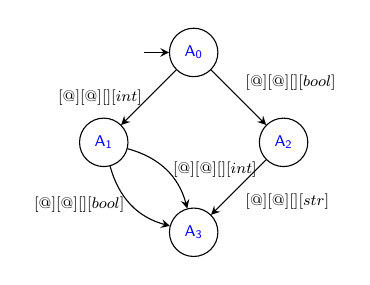
\begin{tikzpicture}[mycfsm,initial where=left,scale=.7]
        \node[state,initial] (A0) {$\ptp[A_0]$};
        \node[state, below left=of A0] (A1)  {$\ptp[A_1]$};
        \node[state, below right=of A0] (A2)  {$\ptp[{A_2}]$};
        \node[state, below left=of A2] (A3)  {$\ptp[{A_3}]$};
        %
        \path
        (A0) edge node (a01) [left] {$\aout[@][@][][int]$} (A1)
        (A0) edge node {$\aout[@][@][][bool]$} (A2)
        (A1) edge [bend left] node  [right] {$\aout[@][@][][int]$} (A3)
        (A1) edge [bend right] node (a13) [left] {$\aout[@][@][][bool]$} (A3)
        (A2) edge node  {$\aout[@][@][][str]$} (A3)
        % (A3) edge [loop below] node [below] {$\ain[\q][\p][][{\msg[bool]}]$} (A3)
        ;
      \end{tikzpicture}
      &
      \uncover<2->{
        \begin{tabular}{c}
          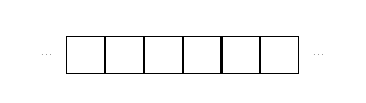
\begin{tikzpicture}[scale=0.4, every node/.style={transform shape}]
            \begin{scope}[start chain=1 going right,node distance=0.2mm]
              \node [on chain=1,tmtape,draw=none] {$\ldots$};
              \node [on chain=1,tmtape] (xx) {};
              \node [on chain=1,tmtape] (input) {};
              \node [on chain=1,tmtape] {};
              \node [on chain=1,tmtape] {};
              \node [on chain=1,tmtape] (abb) {};
              \node [on chain=1,tmtape] (aba) {};
              \node [on chain=1,tmtape,draw=none] {$\ldots$};
              \onslide<1-4>{\node[above=of aba, font=\LARGE] (arrowtopa) {$\blacktriangledown$};}
              % \onslide<1-4>\draw[line] (arrowtopa) -- (aba);
              %
              \onslide<5->{\node[above=of abb, font=\LARGE] (arrowtopb) {$\blacktriangledown$};}
              % \onslide<5->{\draw[line] (arrowtopb) -- (abb);}
            \end{scope}
          \end{tikzpicture}
          \\[.4cm]
          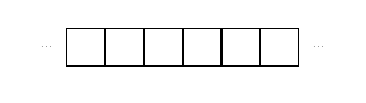
\begin{tikzpicture}[scale=0.4, every node/.style={transform shape}]
            \begin{scope}[start chain=1 going right,node distance=0.2mm]
              \node [on chain=1,tmtape,draw=none] {$\ldots$};
              \node [on chain=1,tmtape] (baa) {};
              \node [on chain=1,tmtape] (input) {};
              \node [on chain=1,tmtape] (ba8) {};
              \node [on chain=1,tmtape] (ba9) {};
              \node [on chain=1,tmtape] (ba10) {};
              \node [on chain=1,tmtape] (ba11) {};
              \node [on chain=1,tmtape,draw=none] {$\ldots$};
              %
              \node [below=of baa] (arrowbot) {$\blacktriangle$};
              % \draw[line] (arrowbot) -- (baa);
            \end{scope}
          \end{tikzpicture}
        \end{tabular}
      }
      &
      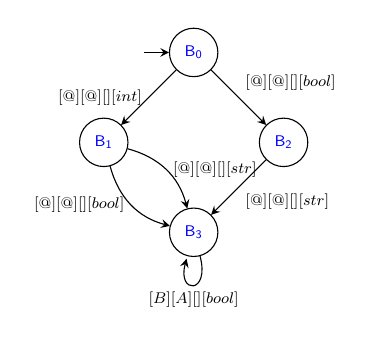
\begin{tikzpicture}[mycfsm,initial where=left, scale=.7]
        \node[state,initial] (A0) {$\ptp[{B_0}]$};
        \node[state, below left=of A0] (A1)  {$\ptp[{B_1}]$};
        \node[state, below right=of A0] (A2)  {$\ptp[{B_2}]$};
        \node[state, below left=of A2] (A3)  {$\ptp[{B_3}]$};
        %
        \path
        (A0) edge node (b01) [left] {$\ain[@][@][][int]$} (A1)
        (A0) edge node  {$\ain[@][@][][bool]$} (A2)
        (A1) edge [bend left] node  [right] {$\ain[@][@][][str]$} (A3)
        (A1) edge [bend right] node (b13) [left] {$\ain[@][@][][bool]$} (A3)
        (A2) edge node  {$\ain[@][@][][str]$} (A3)
        (A3) edge [loop below] node (b33) [below] {$\aout[B][A][][bool]$} (A3)
        ;
      \end{tikzpicture}
      \\
      $\p$ & & $\q$
    \end{tabular}
  \end{center}
  \begin{tikzpicture}[overlay]
  %
  \node<2-4>[font=\tiny] at ($(aba)!0.5!(aba)$) {$\msg[int]$};
  \node<3-5>[font=\tiny] at ($(abb)!0.5!(abb)$) {$\msg[bool]$};
  %
  \node<6->[font=\tiny] at ($(baa)!0.5!(baa)$) {$\msg[bool]$};
  \node<7->[font=\tiny] at ($(input)!0.5!(input)$) {$\msg[bool]$};
  \node<8->[font=\tiny] at ($(ba8)!0.5!(ba8)$) {$\msg[bool]$};
  % \node<9->[font=\tiny] at ($(ba9)!0.5!(ba9)$) {$\msg[bool]$};
  % \node<10->[font=\tiny] at ($(ba10)!0.5!(ba10)$) {$\msg[bool]$};
  % \node<11->[font=\tiny] at ($(ba11)!0.5!(ba11)$) {$\msg[bool]$};
  %
  \node<2-8>[rectangle, fill=\newgreen!30, fit=(a01), inner sep=0pt, opacity=0.2] {};
  \node<2-3>[rectangle, fill=\newgreen, fit=(aba),inner sep=0pt,opacity=0.2] {};
  \node<3-8>[rectangle, fill=\newgreen, fit=(a13),inner sep=0pt,opacity=0.2] {};
  \node<3-3>[rectangle, fill=\newgreen, fit=(abb),inner sep=0pt,opacity=0.2] {};
  \node<4->[rectangle, fill=yellow!60, fit=(b01),inner sep=0pt,opacity=0.2] {};
  \node<4-4>[rectangle, fill=yellow!60, fit=(aba),inner sep=0pt,opacity=0.2] {};
  \node<5->[rectangle, fill=yellow!60, fit=(b13),inner sep=0pt,opacity=0.2] {};
  \node<5-5>[rectangle, fill=yellow!60, fit=(abb),inner sep=0pt,opacity=0.2] {};
  \node<6->[rectangle, fill=yellow!60, fit=(b33),inner sep=0pt,opacity=0.2] {};
  \node<6->[rectangle, fill=yellow!60, fit=(baa),inner sep=0pt,opacity=0.2] {};
  % \node<8-8>[rectangle, fill=\newgreen, fit=(b33),inner sep=0pt,opacity=0.2] {};
  \node<7->[rectangle, fill=yellow!60, fit=(input),inner sep=0pt,opacity=0.2] {};
  \node<8->[rectangle, fill=yellow!60, fit=(ba8),inner sep=0pt,opacity=0.2] {};
  % \node<9->[rectangle, fill=yellow!60, fit=(ba9),inner sep=0pt,opacity=0.2] {};
  % \node<9->[rectangle, fill=yellow!60, fit=(ba9),inner sep=0pt,opacity=0.2] {};
  % \node<10->[rectangle, fill=yellow!60, fit=(ba10),inner sep=0pt,opacity=0.2] {};
  % \node<11->[rectangle, fill=yellow!60, fit=(ba11),inner sep=0pt,opacity=0.2] {};
  % \node<10-10>[rectangle, fill=yellow!60, fit=(b33),inner sep=0pt,opacity=0.2] {};
  % \node<11-11>[rectangle, fill=yellow!60, fit=(b33),inner sep=0pt,opacity=0.2] {};
\end{tikzpicture}
}%%%end cfsmanimation

\newcommandx{\choranimation}[2][1=1,2=1,usedefault=@]{
  \begin{overlayarea}{#1\linewidth}{#2\textheight}
    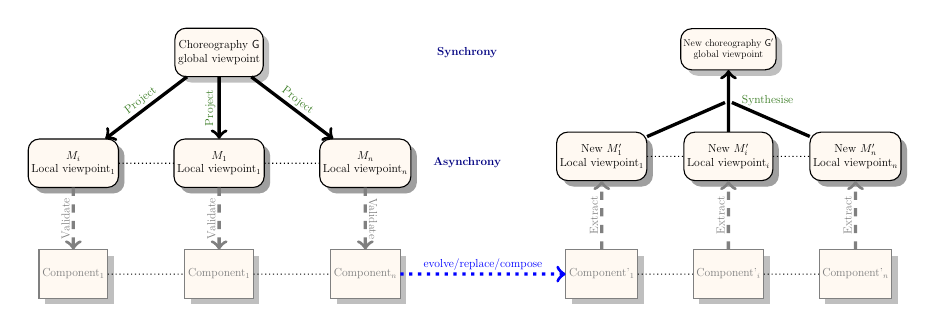
\begin{tikzpicture}[
      node distance=1cm and 2cm,
      scale=0.35,
      every node/.style={transform shape},
      font=\large
      ]
      \node [choreo, align=center] (global){Choreography $\aG$ \\ global viewpoint};
      %
      \node [below= of global] (fake) {};
      \node<2-> (synctxt) at (9,0)  {\textcolor{NavyBlue}{\bf Synchrony}};
      % 
      \node [choreo, align=center, local, below =of fake] (typei) {$\aCM_1$ \\ Local viewpoint$_1$};
      \node [choreo, align=center, local, left =of typei] (type1) {$\aCM_i$ \\ Local viewpoint$_1$};
      \node [choreo, align=center, local, right=of typei] (typen) {$\aCM_n$ \\ Local viewpoint$_n$};
      \node<2-> (asynctxt) at (9,-4) {\textcolor{NavyBlue}{\bf Asynchrony}};
      %
      \node<2-> [below=of type1] (fake1) {};
      \node<2-> [below=of typei] (fakei) {};
      \node<2-> [below=of typen] (faken) {};
      % 
      \node<3-> [process, below=of fake1] (proc1) {Component$_1$};
      \node<3-> [process, below=of fakei] (proci) {Component$_1$};
      \node<3-> [process, below=of faken] (procn) {Component$_n$};
      %
      \node<4-> [process, right=of procn,xshift=4cm] (evolve1) {Component'$_1$};
      \node<4-> [process, right=of evolve1] (evolvei) {Component'$_i$};
      \node<4-> [process, right=of evolvei] (evolven) {Component'$_n$};
      % 
      \node<5-> [choreo, align=center, local, above=of evolve1, yshift=1.5cm] (t11) {New $\aCM'_1$ \\ Local viewpoint$_1$};
      \node<5-> [choreo, align=center, local, above=of evolvei, yshift=1.5cm] (t1i) {New $\aCM'_i$ \\ Local viewpoint$_i$};
      \node<5-> [choreo, align=center, local, above=of evolven, yshift=1.5cm] (t1n) {New $\aCM'_n$ \\ Local viewpoint$_n$};
      %
      \node<6> [above=of t1i, yshift=1.5cm] (qm) {\Huge \textcolor{red}{ ??? }};
      \node<6-> [above=of t1i] (dummy) {};
      \node<7-> [choreo,align=center,above=of dummy,scale=.85] (global') {New choreography $\aG'$ \\ global viewpoint};
      %
      \path<3-> [bigar,->,dashed,gray] (type1) edge[sloped,above] node {Validate} (proc1);
      \path<3-> [bigar,->,dashed,gray] (typei) edge[sloped,above] node {Validate} (proci);
      \path<3-> [bigar,->,dashed,gray] (typen) edge[sloped,above] node {Validate} (procn);
      %
      \path<2-> [bigar] (global) edge[sloped,above] node {\color{OliveGreen}Project} (type1);
      \path<2-> [bigar] (global) edge[sloped,above] node {\color{OliveGreen}Project} (typei);
      \path<2-> [bigar] (global) edge[sloped,above] node {\color{OliveGreen}Project} (typen);
      % 
      \path<2-> [elli] (type1) -- (typei);
      \path<2-> [elli] (typei) -- (typen);
      % 
      \path<3-> [elli] (proc1) -- (proci);
      \path<3-> [elli] (proci) -- (procn);
      %
      \path<4-> [bigar,blue,dotted] (procn) edge node [above] {evolve/replace/compose} (evolve1);      
      \path<4-> [elli] (evolve1) -- (evolvei);
      \path<4-> [elli] (evolvei) -- (evolven);
      %
      \path<5-> [elli] (t11) -- (t1i);
      \path<5-> [elli] (t1i) -- (t1n);
      %
      \path<5-> [bigar,->,dashed,gray] (evolve1) edge[sloped,above] node {Extract} (t11);
      \path<5-> [bigar,->,dashed,gray] (evolvei) edge[sloped,above] node {Extract} (t1i);
      \path<5-> [bigar,->,dashed,gray] (evolven) edge[sloped,above] node {Extract} (t1n);
      %
      \path<7-> [bigar,-] (t11) -- (dummy);
      \path<7-> [bigar,->] (t1i) edge node[right,xshift=1em] {\color{OliveGreen}Synthesise} (global');
      \path<7-> [bigar,-] (t1n) -- (dummy);
    \end{tikzpicture}
  \end{overlayarea}
}%%%end choranimation

\newcommand{\cempty}{\mathbf{[]}}
\newcommandx{\cm}[2][1=\ptp, 2=\aM]{{#2}_{#1}}
% \newcommandx{\achan}[2][1=A,2=B,usedefault=@]{\overset{\to}{\ptp[{#1}]\,\ptp[{#2}]}}
\newcommandx{\achan}[2][1=A,2=B,usedefault=@]{{\ptp[#1]}{\,}{\ptp[#2]}}
\newcommand{\ptpset}{\mathcal{\colorPtp{P}}}
\newcommand{\PSet}{\ptpset}
\newcommand{\pset}{\ptpset}
\newcommand{\chan}[1]{\ptp[#1]}
\newcommand{\ASigma}{\msgset}
\newcommand{\oact}{\outop[]}
\newcommand{\iact}{\inop[]}
\newcommand{\tset}{\to}
\newcommand{\Smv}{\vec{S}}
\newcommand{\csconf}[2]{\conf{\vec{#1} \ ; \ \vec{#2}}}
\newcommand{\chanset}{\chset}
\newcommand{\TRANSS}[1]{{\xRightarrow{\raisebox{-.3ex}[0pt][0pt]{$\scriptstyle #1$} }}}
\newcommand{\RS}[1][]{\mathsf{RC}_{#1}}
\newcommand{\NUL}{\boldsymbol{}\varepsilon}
\newcommand{\asend}[3]{\ptp{#1} \! \rightarrowtriangle \! \ptp{#2} \!:\! \mbox{$\ptp{#3}$}}
\newcommand{\chosyn}{\chorgram}
\newcommand{\dirpoms}{\toolid{DirPoms}}
\newcommand{\trans}[2][{}]{\,\xrightarrow{#2}_{#1}\,}
\newcommand{\cint}{\gint[{}]}
\newcommand{\cfsmTS}[1][0]{\mathit{TS}_{#1}}
\newcommandx{\acfsmout}[3][1=A,2=B,3=m,usedefault=@]{\achan[{#1}][{#2}] \oact {\msg[{#3}]}}
\newcommandx{\acfsmin}[3][1=A,2=B,3=m,usedefault=@]{\achan[{#1}][{#2}] \iact {\msg[{#3}]}}
\newcommandx{\fsaout}[2][1={\p},2={},usedefault=@]{
  \ptp[#1] \ \outop[]\ \msg[{#2}]
}
\newcommandx{\fsain}[2][1={\p},2={},usedefault=@]{
  \ptp[#1] \ \inop[]\ \msg[{#2}]
}

\makeatletter
\newcommand{\linenumfontsize}{\@setfontsize{\linenumfontsize}{3pt}{3pt}}
\makeatother
\lstset{
  numbers=left,
  numberstyle=\linenumfontsize,
  backgroundcolor=\color{black!3},
  basicstyle=\sffamily\tiny,
  tabsize=3,
  mathescape=true,
  morekeywords={of,do,system,||},
  morecomment=[l]{..},
  morecomment=[s]{[}{]},
  commentstyle=\color{blue!80!red!40},
  literate=*{=}{{\colorOp}{=}}{1}{||}{{\colorOp{||}}}{1}{+}{{\colorOp{+}}}{1}{!}{{\colorOpForestGreen}{!}}{1}{?}{{\colorOp{?}}}{1}{;}{{\colorOp{;}}}{1},
  keywordstyle=\color{ForestGreen}
 }

\lstdefinelanguage{sys}{
	commentstyle=\color{Gray},
%	morecomment=[l]{..},
	morecomment=[s]{[}{]},
   % keywordsprefix={receive},
	keywords=[0]{system,of,do,end},	keywordstyle=\color{orange}\bfseries,
%	morekeywords=[1]{\*,\+,\!,\?,\|,\=},	keywordstyle=[1]\color{blue}\bfseries,
}

\newcommand{\participant}[1]{\p[#1]}
\newcommand{\payload}[1]{$\msg[#1]$}
\lstdefinelanguage{sgg}{
  commentstyle=\color{Gray},
  morecomment=[l]{..},
  morecomment=[s]{[}{]},
  keywords=[0]{repeat,branch,sel},
  keywordstyle=\color{orange}\bfseries,
  morekeywords=[1]{*,\+,|,->},
  literate={->}{$\colorOp \xrightarrow$}1 {|}{$\gparop$}1 {;}{$\gseqop$}1 {+}{$\gchoop$}1 {\{}{{\textcolor{NavyBlue}{\{}}}1 {\}}{{\textcolor{NavyBlue}{\}}}}1
}

%%%%%%%%%%%%%%%%%%%%%%%%%%%%%%%%%%%%%%%%%%%%%%%%%%%%%%%%%%%%%%%%%%%%%%%%%%%%%
%%%                        END CFSM MACROS                                %%%
%%%%%%%%%%%%%%%%%%%%%%%%%%%%%%%%%%%%%%%%%%%%%%%%%%%%%%%%%%%%%%%%%%%%%%%%%%%%%




%%%%%%%%%%%%%%%%%%%%%%%%%%%%%%%%%%%%%%%%%%%%%%%%%%%%%%%%%%%%%%%%%%%%%%%%%%%%%
%%%                          GRAPHS MACROS                                %%%
%%%%%%%%%%%%%%%%%%%%%%%%%%%%%%%%%%%%%%%%%%%%%%%%%%%%%%%%%%%%%%%%%%%%%%%%%%%%%
\newcommand{\aG}{\mathsf{G}}
\newcommand{\gsink}{\circledcirc}
\newcommand{\gsource}{\circ}
\newcommand{\gvertex}{\bullet}
\newcommand{\gseqop}{{\colorOp ;}\,}
\newcommand{\gparop}{{\colorOp \ |\ }}
\newcommand{\gchoop}{{\colorOp \ +\ }}
\newcommand{\grecop}{{\colorOp *}}
\newcommand{\grecopp}{{\colorOp{@}}}
\newcommandx{\nmerge}[2][1={i},2={},usedefault=@]{
  \ifempty{#2}{
    \ifempty{#1}{\mu}{\gname[-{#1}]}
  }{-{#2}}
}

\newcommand{\gselkw}{\textcolor{OliveGreen}{\mathtt{sel}}}
\newcommand{\grepkw}{\textcolor{OliveGreen}{\mathtt{repeat}}}
\newcommand{\gblk}[1][\aG]{\textcolor{NavyBlue}{\{} #1 \textcolor{NavyBlue}{\}}}
\newcommandx{\intpar}[2][1={\aint},2={\aint[b]},usedefault=@]{{#1}\parallel{#2}}

\mkfun{\cuui}{cui}{\clang}
\mkfun{\cuuiasym}{cui${^\textit{asym}}$}{\clang}
% \newcommand{\esbj}[1][\ae]{{\colorFun{\textsf{sbj}\ifempty{#1}{}{(#1)}}}}
\mkfun{\esbj}{sbj}{\ae}
\newcommand{\esubject}{\esbj}
\makeatletter%
\@ifclassloaded{exam-paper}%
  {}%
  {\makeatletter%
    \@ifclassloaded{test}%
    {}%
%    {\newcommand{\subject}{\esbj}}%
    \makeatother%
  }
\makeatother%


\newcommandx{\gnode}[2][1=i,2=\gint,usedefault=@]{
  \ifcp{
    \ifempty{#1}{#2}{\gname[#1].\big({#2}\big)}
  }
  \else
  {#2}
  \fi
}
   
\newcommand{\cpset}{\mathbb{\colorNode{Z}}_0}
\newcommand{\nodeset}{\cpset}
\newcommand{\gempty}{\mathbf{0}}
\newcommandx{\gint}[4][1=i,2=A,3=m,4=B,usedefault=@]{
  \scalebox{.8}{$
	 \ptp[#2] {\colorOp \xrightarrow{\scriptstyle \gname[#1]}} \ptp[#4] \! {\colorOp \colon} \! \!{\msg[{#3}]}
  $}
}
% \newcommandx{\gint}[4][1=i,2=A,3=m,4=B,usedefault=@]{
%   \ptp[#2] {\colorOp \xrightarrow{\scriptstyle \gname[#1]}} \ptp[#4]\ \!\!\! {\colorOp \colon} \!\!{\msg[{#3}]}
% }
\newcommandx{\gout}[4][1=\gname,2=\ptp,3=m,4={\ptp[C]},usedefault=@]{
  \achan[{#2}][{#4}] {\colorOp {\colorOp{!}}} {\msg[{#3}]}
}
\newcommandx{\gin}[4][1=\gname,2=\ptp,3=m,4={\ptp[C]},usedefault=@]{
  \achan[{#2}][{#4}] {\colorOp {\colorOp{?}}} {\msg[{#3}]}
}
\newcommandx{\gseq}[3][1=\gname,2={\aG},3={\aG'},usedefault=@]{
  \def\ggraph{{#2} \gseqop {#3}}
  \ggraph
}
\newcommand{\ginfix}[4]{
  \def\ggraph{{#2} {#4} {#3}}
  \gnode[#1][\ggraph]
}
\newcommandx{\gpar}[3][1=i,2={\aG},3={\aG'},usedefault=@]{
  \ginfix{#1}{#2}{#3}{\gparop}
}
\newcommandx{\gcho}[3][1=i,2={\aG},3={\aG'},usedefault=@]{
  \ginfix{#1}{#2}{#3}{\gchoop}
}
\newcommandx{\gchov}[3][1=\gname,2={\aG},3={\aG'},usedefault=@]{
  \def\ggraph{\left(
  \begin{array}l
    \ifempty{#1}{{#2} \\ \gchoop \\ {#3}}{\!\!{#2} \\ \gchoop \\ {#3}}
  \end{array}\right)}
  \ifcp\gnode[{$#1$}][\ggraph] \else \ggraph \fi
}
\newcommandx{\grec}[3][1=i,2={\aG},3={\p},usedefault=@]{
  \def\ggraph{\grecop {#2} \ifempty{#3}{}{\grecopp {#3}}}
  \ifempty{#1}{\ggraph}{\gname[{$#1$}][\ggraph]}
}	

\newcommand{\getcentroid}[2]{
    \coordinate (tmpgatecoord) at (0,0);
    \foreach \n [count=\i] in {#1}{
      \path (\n);
      \coordinate (tmpgatecoord) at ($(tmpgatecoord) + (\n)$);
      \coordinate (#2) at ($1/\i*(tmpgatecoord)$);
      %\node at (#2) {#2};
    }
}


\tikzset{
  hgsem/.style={
    draw,
    node distance=2cm and 1cm,
    transform shape,
    smooth,
    every node/.style = {font=\sffamily\bfseries}
  }
}

\tikzset{
  hgstyle/.style={
    src color={#1},
    tgt color={#1},
    centroid color={#1},
    centroid label={#1},
    centroid name={#1},
    centroid radius={#1},
    centroid ratio={#1},
    xoffset={#1},
    yoffset={#1},
    xsrcoffset={#1},
    ysrcoffset={#1},
    xtgtoffset={#1},
    ytgtoffset={#1},
    font={#1},
    centroid angle={#1},
    centroid tolerance={#1}
  },
  %
  src color/.store in = \hgsrccol,
  tgt color/.store in = \hgtgtcol,
  centroid color/.store in =\hgfillcolor,
  centroid label/.store in =\hglabel,
  centroid name/.store in =\hgname,
  centroid radius/.store in = \hgradius,
  centroid ratio/.store in = \hgratio,
  xoffset/.store in =\hgxoffset,
  yoffset/.store in =\hgyoffset,
  xsrcoffset/.store in =\hgxsrcoffset,
  ysrcoffset/.store in =\hgysrcoffset,
  xtgtoffset/.store in =\hgxtgtoffset,
  ytgtoffset/.store in =\hgytgtoffset,
  centroid angle/.store in =\hgangle,
  centroid tolerance/.store in =\hgtolerance,
  % 
  src color = black,
  tgt color = black,
  centroid color = orange!40,
  centroid label={},
  centroid name={dummycentroid},
  centroid radius = .7pt,
  centroid ratio = .35,
  xoffset = 0,
  yoffset = 0,
  xsrcoffset = 0,
  ysrcoffset = 0,
  xtgtoffset = 0,
  ytgtoffset = 0,
  font=\sffamily\scriptsize,
  centroid angle=0,
  centroid tolerance=10pt
}

\newcommandx{\mkhg}[5][1={},4={},5={},usedefault=@]{
  \begingroup
  \tikzset{#1}
  \StrCount{#2,}{,}[\l] % from package xxstring
  \StrCount{#3,}{,}[\m] % from package xxstring
  \ifthenelse{\l = 1 \AND \m = 1}{
    \ifempty{#4}{
      \ifempty{#5}{
        \path[hgsem, ->, >=stealth', shorten >=1pt] (#2) -- (#3);
      }{
        \path[hgsem, ->, >=stealth', shorten >=1pt] (#2) #5 (#3);
      }
    }{
      \ifempty{#5}{
        \path[hgsem, ->, >=stealth', shorten >=1pt, #4] (#2) -- (#3);
      }{
        \path[hgsem, ->, >=stealth', shorten >=1pt, #4] (#2) #5 (#3);
      }
    }
  }{
    \coordinate (srcoffset) at (\hgxsrcoffset,\hgysrcoffset);
    \coordinate (tgtoffset) at (\hgxtgtoffset,\hgytgtoffset);
    \getcentroid{#2}{srccentroid};
    \getcentroid{#3}{tgtcentroid};
    \node[label={left:\hglabel}] (\hgname) at ($(srccentroid)!{1-\hgratio}!\hgangle:(tgtcentroid) + (\hgxoffset,\hgyoffset)$) {};
    \pgfgetlastxy \xc \yc;
    \pgfmathtruncatemacro{\xcontrol}{\xc};
    \pgfmathtruncatemacro{\ycontrol}{\yc};
    \foreach \n in {#2}{
      \path (\n);
      \pgfgetlastxy \xntmp \yntmp;
      \pgfmathtruncatemacro{\xn}{\xntmp};
      \pgfmathtruncatemacro{\yn}{\yntmp};
      \pgfmathsetmacro\xtmpdiff{abs(\xn - \xcontrol + \hgxsrcoffset)};
      \pgfmathsetmacro\ytmpdiff{abs(\yn - \ycontrol + \hgytgtoffset)};
      \ifdim \xtmpdiff pt > \hgtolerance
      \ifempty{#4}{
        \path[hgsem, \hgsrccol] (\n) .. controls ($(srccentroid.center) + (srcoffset)$) .. (\hgname.center);
      }{
        \path[hgsem, \hgsrccol] (\n) .. controls ($(srccentroid.center) + (srcoffset)$) .. (\hgname.center);
      }
      \else
      \ifempty{#4}{
        \path[hgsem, \hgsrccol] (\n) -- (\hgname.center);
      }{
        \path[hgsem, \hgsrccol, #4] (\n) -- (\hgname.center);
      }
      \fi
    }
    \foreach \n in {#3}{
      \path (\n);
      \pgfgetlastxy \xntmp \yntmp;
      \pgfmathtruncatemacro{\xn}{\xntmp};
      \pgfmathtruncatemacro{\yn}{\yntmp};
      \pgfmathsetmacro\xtmpdiff{abs(\xn - \xcontrol)};
      \pgfmathsetmacro\ytmpdiff{abs(\yn - \ycontrol)};
      \ifdim \xtmpdiff pt > \hgtolerance
      \ifempty{#4}{
        \path[hgsem, ->, >=stealth', shorten >=1pt, \hgtgtcol] (\hgname.center) .. controls (tgtcentroid.center) and ($(tgtcentroid.center) + (tgtoffset)$) .. (\n);
      }{
        \path[hgsem, ->, >=stealth', shorten >=1pt, \hgtgtcol,#4] (\hgname.center) .. controls (tgtcentroid.center) and ($(tgtcentroid.center) + (tgtoffset)$) .. (\n);
      }
      \else
      \ifempty{#4}{
        \path[hgsem, ->, >=stealth', shorten >=1pt, \hgtgtcol] (\hgname.center) --  (\n);
      }{
        \path[hgsem, ->, >=stealth', shorten >=1pt, \hgtgtcol] (\hgname.center) --  (\n);
      }
      \fi
    }
    \fill[\hgfillcolor] (\hgname) circle [radius=\hgradius];
  }
  \endgroup
}

\newcommand{\hghb}[1]{\widehat{#1}}
\newcommandx{\hgordeq}[1][1={\aH},usedefault=@]{\sqsubseteq_{#1}}
%
\newcommandx{\gintsem}[4][4=.5]{
  \tikz[hgsem,scale=#4,every node/.style={font=\scriptsize}]{
    \node (out) {$\aout[{#1}][{#2}][][{#3}]$};
    \node[below = 20pt of out] (in) {$\ain[{#1}][{#2}][][{#3}]$};
    \mkhg{out}{in};
  }
}

% \newcommandx{\gsem}[2][1={\aG},2={},usedefault=@]{\left[\!\left[ {#1} \right]\!\right]_{#2}}
\newcommandx{\gsem}[2][1={\aG},2={},usedefault=@]{\left\llbracket {#1} \right\rrbracket_{#2}}

\newcommandx{\rbot}{\text{undef}}
\newcommandx{\rtrs}[1][1={\aH},usedefault=@]{{#1}^{\star}}
\newcommandx{\gord}[1][1={\aG},usedefault=@]{\leq_{#1}}
\newcommandx{\gordeq}[1][1={\aG},usedefault=@]{\leq_{#1}}
\mkfun{\cause}{cs}{}
\mkfun{\effect}{ef}{}
% \newcommandx{\efst}[1]{\textsf{cs}\ifempty{#1}{}{_{({#1})}}}
\newcommand{\hgflattening}[1]{\widehat{#1}}


%%%%%%%%%%%%%%%%%%%%%%%%%%%%%%%%%%%%%%%%%%%%%%%%%%%%%%%%%%%%%%%%%%%%%%%%%%%%%
%%%                      END GRAPHS MACROS                                %%%
%%%%%%%%%%%%%%%%%%%%%%%%%%%%%%%%%%%%%%%%%%%%%%%%%%%%%%%%%%%%%%%%%%%%%%%%%%%%%

%to remove
\newcommandx{\aW}{w}
%\newcommandx{\rlang}{\mathcal{L}}
\newcommand{\clang}{\mathcal{\colorLang L}}
\newcommand{\alang}{\mathbb{\colorLang L}}
%\newcommand{\enode}[1]{{\colorAct{\textsf{cp}}\ifempty{#1}{}{({#1})}}}
% \newcommand{\eact}[1]{{\colorAct{\textsf{act}}}\ifempty{#1}{}{({#1})}}
\newcommand{\gfun}[1]{\ensuremath{\mathsf{\colorFun #1}}}
\mkfun{\eact}{\gfun{act}}{}
\mkfun{\enode}{\gfun{cp}}{}

\mkuop{\rmax}{\gfun{max}}{\aH}
\mkuop{\rmin}{\gfun{min}}{\aH}
\mkuop{\rMAX}{\gfun{lst}}{\aH}
\mkuop{\rMIN}{\gfun{fst}}{\aH}
\newcommand{\rlt}[1][\aH]{<_{#1}}
\newcommandx{\rseq}[2][1=\aG,2={\aG'},usedefault=@]{\gfun{seq}({#1},{#2})}
\newcommandx{\rpar}[2][1=\aG,2={\aG'},usedefault=@]{\gfun{par}({#1},{#2})}

\newcommandx{\gproj}[2][1=\aG,2=\ptp]{{#1}\downarrow_{#2}}
\newcommandx{\cinit}[1][1={\aQzero},usedefault=@]{{#1}}
\newcommandx{\cfinal}[1][1={q_e},usedefault=@]{{#1}}
\newcommand{\ctr}[3]{
  \tikz{
    \node at (0,0) (i) {};
    \node[shape=circle,draw,inner sep=1pt] at (0.6,0) (s) {$#1$};
    \node[shape=circle,draw,inner sep=1pt, right=of s] at (1.7,0)  (t) {$#2$};
    \node at (3.2,0) (f) {};
    \draw[->] (i) -- (s);
    \draw[->] (s) -- (t) node [midway,above]{$#3$};
    \draw[->] (t) -- (f);
  }
}
\newcommand{\ccup}{\sqcup}
\newcommand{\ccap}{\cap}
\newcommand{\cprod}{\otimes}
\newcommandx{\geproj}[4][1=\aG,2=\ptp,3=\cinit,4=\cfinal,usedefault=@]{
  {#1}\downarrow_{#2}^{{#3},{#4}}
}

\newcommand*{\StrikeThruDistance}{0.15cm}%
\newcommand*{\StrikeThru}{\StrikeThruDistance,\StrikeThruDistance}%
\tikzset{strike thru arrow/.style={
    decoration={markings, mark=at position 0.5 with {
        \draw [blue, thick,-] 
            ++ (-\StrikeThruDistance,-\StrikeThruDistance) 
            -- ( \StrikeThruDistance, \StrikeThruDistance);}
    },
    postaction={decorate},
}}


\newcommandx{\ich}[1][1={\aG},usedefault=@]{{#1}^{\oplus}}
\newcommandx{\ichedges}[2][1={\aG},2={\gname},usedefault=@]{{#1}^{\oplus}({#2})}
\newcommandx{\parts}[1]{2^{#1}}
\newcommandx{\actch}{c}
\newcommandx{\soundactch}[2][1={\aG},2={\actch},usedefault=@]{{#1} \,\circledR\, {#2}}
\newcommandx{\rOnActch}[2][1={\aG},2={\actch},usedefault=@]{{#1} \setminus {#2}}
\newcommandx{\rOnActchClean}[2][1={\aG},2={\actch},usedefault=@]{{#1} \circledR {#2}}
\newcommandx{\rAllEvents}[1][1={\aG},usedefault=@]{\mathit{dom}(#1)}

\newcommand{\av}{\ae}
\newcommand{\aV}{\aE}
\newcommand{\AV}{\mathcal{V}}
\newcommand{\aH}{H}
\newcommand{\ah}{h}
\newcommandx{\hgvertex}[2][1=\al,2=\gname,usedefault=@]{{#1}_{\textcolor{red}{[{#2}]}}}
\newcommand{\aE}{{\colorE E}}
\renewcommand{\ae}[1][e]{{\colorE{#1}}}
\newcommand{\aL}{{\tilde \al}}
\newcommand{\al}[1][l]{{\colorE{#1}}}
\newcommandx{\hyedge}[1]{\{#1\}}

\newcommandx{\rdiv}[2][1=\gcho,2=\ptp,usedefault=@]{
  \gfun{div}_{#2}(#1)
}

\newcommandx{\rrdiv}[5][1={\aG},2={\aG'},3={\AV},4={,\AV'},5=\ptp,usedefault=@]{
  \gfun{div}^{#3#4}_{#5}(#1,#2)
%#1 \xhookleftarrow{#3} \!\!{_{#5}} \!\!\xhookrightarrow{#4} #2
}
\newcommandx{\pdiv}[3][1={\apom_1},2={\apom_2},3={\apom},usedefault=@]{
  \gfun{div}_{#3}(#1,#2)
%#1 \xhookleftarrow{#3} \!\!{_{#5}} \!\!\xhookrightarrow{#4} #2
}
\newcommandx{\pfork}[3][1={\apom_1},2={\apom_2},3={\apom},usedefault=@]{
  \gfun{fork}_{#3}(#1,#2)
%#1 \xhookleftarrow{#3} \!\!{_{#5}} \!\!\xhookrightarrow{#4} #2
}

%%%%%%%%%%%%%%%%%%%%%%%%%%%%%%%%%%%%%%%%%%%%%%%%%%%%%%%%%%%%%%%%%%%%%%%%%%%%%
%%%                            TIKZ MACROS                                %%%
%%%%%%%%%%%%%%%%%%%%%%%%%%%%%%%%%%%%%%%%%%%%%%%%%%%%%%%%%%%%%%%%%%%%%%%%%%%%%

\tikzset{
  pomset/.style={
    node distance = .6cm and .6cm,
    scale = .7,
    transform shape,
    smooth
  }
}


\newcommandx{\mkint}[6][3=i,4=\p,5=\msg,6=\q,usedefault=@]{
%  \node[bblock\ifempty{#1}{}{,{#1}}] \ifempty{#1}{at (0,0)}{} (#2) {$\gint[#3][#4][#5][#6]$};
  \node[bblock, #1] (#2) {$\gint[#3][#4][#5][#6]$};
}

\newcommand{\mkseq}[2]{\path[line] (#1) -- (#2);}

\newcommand{\mknseq}[1]{
  \StrCount{#1}{,}[\l] % from package xxstring
  \StrBefore{#1}{,}[\myhead]
  \StrBehind{#1}{,}[\mytail]
  \StrBefore{\mytail}{,}[\sndel]
  \ifnum \l > 1 {
    \mkseq{\myhead}{\sndel};
    \mknseq{\mytail}
  }
  \else{\ifnum \l > 0{
      \mkseq{\myhead}{\mytail};
    }
    \else{}
    \fi
  }
  \fi
}

\newcommandx{\mkgateblock}[6][6=yellow!10,usedefault=@]{
  % #1: gate
  % #2: position of opening gate
  % #3: comma-separated list of children of opening gate
  % #4: comma-separated list of parents of closing gate
  % #5: position of closing gate
  % #6: background color
  \path(#2);
  \pgfgetlastxy{\xgate}{\ygate};
  \pgfmathtruncatemacro{\xgateround}{\xgate};
  \StrCount{#3,}{,}[\l] % from package xstring
  \ifnum \l < 2 {\errmessage{#3 argument should be a comma-separated list of lenght >= 2}}
  \else{
    \foreach \n in {#3}{
      \path (\n);
      \pgfgetlastxy{\xnode}{\ynode};
      \pgfmathtruncatemacro{\xnround}{\xnode};
      \pgfmathsetmacro\tmpdiff{abs(\xnround - \xgateround)}
      \ifdim \tmpdiff pt > 1 pt \path[line] (#2) -| (\n);
      \else
        \path[line] (#2) -- (\n);
      \fi
    }
  }
  \fi
  \StrCount{#4,}{,}[\l] % from package xstring
  \ifnum \l < 2 {\errmessage{#4 argument should be a comma-separated list of lenght >= 2}}
  \else{
    \foreach \n in {#4}{
      \path (\n);
      \pgfgetlastxy{\xnode}{\ynode};
      \pgfmathtruncatemacro{\xnround}{\xnode};
      \pgfmathsetmacro\tmpdiff{abs(\xnround - \xgateround)}
      \ifdim \tmpdiff pt > 1 pt \path[line] (\n) |- (#5);
      \else
        \path[line] (\n) -- (#5);
      \fi
    }
  }
  \fi
  \node[#1] at (#2) {};
  \node[#1] at (#5) {};
  {
    \begin{pgfonlayer}{background}
      \path[fill=#6,rounded corners]
      (current bounding box.south west) rectangle
      (current bounding box.north east);
    \end{pgfonlayer}
  }
}

\newcommandx{\mkbranchblock}[5][5=@]{
  \mkgateblock{ogate}{#1}{#2}{#3}{#4}[#5]
}

\newcommandx{\mkforkblock}[5][5=@]{
  \mkgateblock{agate}{#1}{#2}{#3}{#4}[#5]
}

\newcommandx{\mkgraph}[3][1=.5cm, usedefault=@]{
  \node[source,above = #1 of {#2}] (src#2) {};
  \node[sink,below  = #1 of {#3}] (sink#3) {};
  \path[line] (src#2) -- (#2);
  \path[line] (#3) -- (sink#3);
}

\newcommandx{\mkloop}[5][1=.5, 2=1.5, 5=\aguard, usedefault=@]{
  % 1: gate position
  % 2: offset back arrow
  % 3: loop start reference
  % 4: loop end reference
  % 6: monitoring guards
  %
  \node[lgate,above = #1 of {#3}] (entry#3) {};
  \pgfgetlastxy \xentry \yentry;
  \pgfmathtruncatemacro{\xentryrounded}{\xentry};
  \node[below = #1 of {#4}, label = {above right:{$#5$}},yshift=-1em] (dummy) {};
  \node[lgate,below  = #1 of {#4}] (exit#4) {};
  \pgfgetlastxy \xexit \yexit;
  \pgfmathtruncatemacro{\xexitrounded}{\xexit};
  \path[line] (entry#3) -- (#3);
  \path[line] (#4) -- (exit#4);
  \pgfmathsetmacro\tmpdiff{abs(\xentryrounded - \xexitrounded)}
  \path[line, color=teal] (exit#4) -| ($(exit#4)+(\tmpdiff,0)+(#2,0)$) |- (entry#3);
}

\newcommandx{\mkfork}[4][2=gatenode,3=i,4=.6,usedefault=@]{
  \mkgatebegin{#1}[{\gname[{#3}]}][agate][#4]{#2}
}

\newcommandx{\mkbranch}[4][2=gatenode,3=i,4=.6,usedefault=@]{
  \mkgatebegin{#1}[{\gname[{#3}]}][ogate][#4]{#2}
}

\newcommandx{\mkgatebegin}[5][2={},3=ogate,4=.5,usedefault=@]{
  % #1: list of nodes
  % #2: control point
  % #3: gate type
  % #4: vertical position offset
  % #5: name of the gate node
  %
  \coordinate (gatecord) at (0,0);
  \coordinate (xmax) at (0,0);
  \coordinate (xmin) at (0,0);
  \pgfgetlastxy \xmin \xmax;
  \foreach \n [count=\i] in {#1}{
    \pgfgetlastxy \xc \yc;
    \path (\n);
    \pgfgetlastxy \xn \yn;
    \ifnum \i = 1
      \coordinate (xmin) at (\xn,0);
      \coordinate (xmax) at (\xn,0);
      \coordinate (max) at (0,\yn);
    \else
      \ifdim \xn < \xmin
        \coordinate (xmin) at (\xn,0);
      \fi
      \ifdim \xn > \xmax
        \coordinate (xmax) at (\xn,0);
      \fi
      \ifdim \yn < \yc
        \coordinate (max) at (0,\yc);
      \else
        \coordinate (max) at (0,\yn);
      \fi
    \fi
  }
  \coordinate (gatecord) at ($(xmin)!.5!(xmax) + (max) + (0,#4) + (max)$);
  \node[#3,label={below:$#2$}] (#5) at (gatecord) {};
  \pgfgetlastxy{\xgate}{\ygate};
  \pgfmathtruncatemacro{\xgateround}{\xgate};
  \StrCount{#1,}{,}[\l] % from package xxstring
  \ifnum \l < 2 {\errmessage{#1 argument should be a comma-separated list of lenght >= 2}}
  \else{
    \foreach \n in {#1}{
      \path (\n);
      \pgfgetlastxy{\xnode}{\ynode};
      \pgfmathtruncatemacro{\xnround}{\xnode};
      \pgfmathsetmacro\tmpdiff{abs(\xnround - \xgateround)}
      \ifdim \tmpdiff pt > 1 pt \path[line] (#5) -| (\n);
      \else
        \path[line] (#5) -- (\n);
      \fi
    }
  }
  \fi
}

\newcommandx{\mkgatebeginold}[5][2={},3=ogate,4=.5,usedefault=@]{
  % #1: list of nodes
  % #2: control point
  % #3: gate type
  % #4: vertical position offset
  % #5: name of the gate node
  %
  \coordinate (gatecord) at (0,0);
  \foreach \n [count=\i] in {#1}{
    \pgfgetlastxy \xc \yc;
    \path (\n);
    \pgfgetlastxy \xn \yn;
    \coordinate (gatecord) at ($(gatecord) + (\xn,0)$);
    \coordinate (gatecord) at ($1/\i*(gatecord)$);
    \ifdim \yn < \yc
    \node (max) at (0,\yc) {};
    \else
    \node (max) at (0,\yn) {};
    \fi
  }
  \coordinate (gatecord) at ($(gatecord) + (0,#4) + (max)$);
  \node[#3,label={below:$#2$}] (#5) at (gatecord) {};
  \pgfgetlastxy{\xgate}{\ygate};
  \pgfmathtruncatemacro{\xgateround}{\xgate};
  \StrCount{#1,}{,}[\l] % from package xxstring
  \ifnum \l < 2 {\errmessage{#1 argument should be a comma-separated list of lenght >= 2}}
  \else{
    \foreach \n in {#1}{
      \path (\n);
      \pgfgetlastxy{\xnode}{\ynode};
      \pgfmathtruncatemacro{\xnround}{\xnode};
      \pgfmathsetmacro\tmpdiff{abs(\xnround - \xgateround)}
      \ifdim \tmpdiff pt > 1 pt \path[line] (#5) -| (\n);
      \else
        \path[line] (#5) -- (\n);
      \fi
    }
  }
  \fi
}

\newcommandx{\mkmerge}[4][2=gatenode,3=i,4=.5,usedefault=@]{
  \mkgateend{#1}[{\ifempty{#3}{}{\nmerge[#3]}}][ogate][#4]{#2}
}

\newcommandx{\mkjoin}[4][2=gatenode,3=i,4=.5,usedefault=@]{\mkgateend{#1}[{\ifempty{#3}{}{\nmerge[#3]}}][agate][#4]{#2}}

\newcommandx{\mkgateend}[5][2={},3=ogate,4=.5,usedefault=@]{
  % #1 list of nodes
  % #2 control point
  % #3 gate type
  % #4 vertical position offset
  % #5 name of the gate node
  %
  \coordinate (gatecord) at (0,0);
  \coordinate (xmax) at (0,0);
  \coordinate (xmin) at (0,0);
  \pgfgetlastxy \xmin \xmax;
  \foreach \n [count=\i] in {#1}{
    \pgfgetlastxy \xc \yc;
    \path (\n);
    \pgfgetlastxy \xn \yn;
    \ifnum \i = 1
      \coordinate (xmin) at (\xn,0);
      \coordinate (xmax) at (\xn,0);
      \coordinate (ymin) at (0,\yn);
    \else
      \ifdim \xn < \xmin
        \coordinate (xmin) at (\xn,0);
      \fi
      \ifdim \xn > \xmax
        \coordinate (xmax) at (\xn,0);
      \fi
      \ifdim \yn > \yc
        \coordinate (ymin) at (0,\yc);
      \else
        \coordinate (ymin) at (0,\yn);
      \fi
    \fi
  }
  \coordinate (gatecord) at ($(xmin)!.5!(xmax) + (ymin)$);
  \node[#3,label={above:$#2$}] (#5) at ($(gatecord) - (0,{#4})$) {};
  \pgfgetlastxy{\xgate}{\ygate};
  \pgfmathtruncatemacro{\xgateround}{\xgate};
  \StrCount{#1,}{,}[\l] % from package xstring
  \ifnum \l < 2 {\errmessage{#1 argument should be a comma-separated list of lenght >= 2}}
  \else{
    \foreach \n in {#1}{
      \path (\n);
      \pgfgetlastxy{\xnode}{\ynode};
      \pgfmathtruncatemacro{\xnround}{\xnode};
      \pgfmathsetmacro\tmpdiff{abs(\xnround - \xgateround)}
      \ifdim \tmpdiff pt > 1 pt \path[line] (\n) |- (#5);
      \else
        \path[line] (\n) -- (#5);
      \fi
    }
  }
  \fi
}

\newcommandx{\mkgateendold}[5][2={},3=ogate,4=.5,usedefault=@]{
  % #1 list of nodes
  % #2 control point
  % #3 gate type
  % #4 vertical position offset
  % #5 name of the gate node
  %
  \coordinate (gatecord) at (0,0);
  \coordinate (xmax) at (0,0);
  \coordinate (xmin) at (0,0);
  \pgfgetlastxy \xmin \xmax;
  \foreach \n [count=\i] in {#1}{
    \pgfgetlastxy \xc \yc;
    \path (\n);
    \pgfgetlastxy \xn \yn;
    \ifdim \xn < \xmin
    \coordinate (xmin) at (\xn,0);
    \fi
    \ifdim \xn > \xmax
    \coordinate (xmax) at (\xn,0);
    \fi
    \ifdim \yn > \yc
    \coordinate (ymin) at (0,\yc);
    \else
    \coordinate (ymin) at (0,\yn);
    \fi
    \coordinate (gatecord) at ($(xmin)!.5!(xmax) + (ymin)$);
  }
  \node[#3,label={above:$#2$}] (#5) at ($(gatecord) - (0,{#4})$) {};
  \pgfgetlastxy{\xgate}{\ygate};
  \pgfmathtruncatemacro{\xgateround}{\xgate};
  \StrCount{#1,}{,}[\l] % from package xstring
  \ifnum \l < 2 {\errmessage{#1 argument should be a comma-separated list of lenght >= 2}}
  \else{
    \foreach \n in {#1}{
      \path (\n);
      \pgfgetlastxy{\xnode}{\ynode};
      \pgfmathtruncatemacro{\xnround}{\xnode};
      \pgfmathsetmacro\tmpdiff{abs(\xnround - \xgateround)}
      \ifdim \tmpdiff pt > 1 pt \path[line] (\n) |- (#5);
      \else
        \path[line] (\n) -- (#5);
      \fi
    }
  }
  \fi
}


\newcommand{\ggateopen}[3][]{
  \ifempty{#1}{}{\path[line] (#1) -- (#2);}
  \foreach \x in {#3} \path[line] (#2) -| (\x);
}

\newcommand{\ggateclose}[3][]{
  \foreach \x in {#3} \path[line] (\x) |- (#2);
  \ifempty{#1}{}{\path[line] (#2) -- (#1);}
}

\newcommand{\gatedistancein}{3pt}
\newcommand{\gatedistanceinand}{2pt}

\usetikzlibrary{
  arrows,
  backgrounds,
  chains,
  calc,
  decorations.markings,decorations.pathreplacing,
  fadings,
  fit,
  patterns,
  petri,
  positioning,
  shadows,
  shapes,automata,shapes.callouts
}

\newcommand{\sourceG}{
  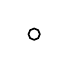
\begin{tikzpicture}[smallglobal,baseline=-.5ex, scale=0.6, every node/.style={transform shape}]
  \node [source] (src) {};
\end{tikzpicture}
}

\newcommand{\sinkG}{
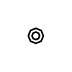
\begin{tikzpicture}[smallglobal,baseline=-.5ex, scale=0.6, every node/.style={transform shape}]
  \node [sink] (src) {};
\end{tikzpicture}
}

\newcommand{\orgateG}{

\begin{tikzpicture}[smallglobal,baseline=-.5ex, scale=0.75, every node/.style={transform shape}]
  \node [ogate] (o) {};
\end{tikzpicture}
}

\newcommand{\lgateG}{

\begin{tikzpicture}[smallglobal,baseline=-.5ex, scale=0.75, every node/.style={transform shape}]
  \node [lgate] (o) {};
\end{tikzpicture}
}

\newcommand{\andgateG}{

\begin{tikzpicture}[smallglobal,baseline=-.5ex, scale=0.75, every node/.style={transform shape}]
  \node [agate] (o) {};
\end{tikzpicture}
}

\tikzset{
  src/.style={draw,circle,fill=white,
    minimum size=2mm,
    inner sep=0pt
  },
  sink/.style={draw,circle,double,fill=white,
    minimum size=1.5mm,
    inner sep=0pt
  },
  node/.style={draw,circle,fill=black,
    minimum size=2mm,
    inner sep=0pt
  },
  % 
  source/.style={draw,circle,fill=white,
    minimum size=3mm,
    inner sep=0pt
  },
  sink/.style={draw,circle,double,fill=white,
    minimum size=3mm,
    inner sep=0pt
  },
  % ACTION
  block/.style = {rectangle, draw=gray, align=center, fill=orange!25, rounded corners=0.1cm,
    minimum size=5mm, inner sep=2pt},
  prenode/.style = {minimum size=9pt,inner sep=2pt, font=\Large},
  % 
  bblock/.style = {rectangle, draw=blue!50, opacity=.7, line width=.5pt, align=center, fill=white, rounded corners=0.1cm,
    minimum size=4mm, inner sep=1pt},
  prenode/.style = {minimum size=9pt,inner sep=2pt, font=\Large},
  % AND GATE
  agate/.style={draw, rectangle,
    minimum size=3mm,
    inner sep=0pt,
    fill=orange!25,
    label={[red]center:$\mid$}
  },
  % ORGATE
  ogate/.style = {
    diamond, draw, fill=orange!25,
    minimum size=4mm,
    inner sep=0pt,
    label={[red]center:$+$}
  },
  % LOOP GATE
  lgate/.style = {
    diamond, draw, fill=orange!25,
    minimum size=4mm,
    inner sep=0pt,
    label={[red]center:$\circlearrowleft$}
    },
  % 
  altogate/.style = {
    diamond, draw,
    minimum size=4mm,
    inner sep=0pt,
    postaction={path picture={% 
        \draw
        ([yshift=\gatedistancein]path picture bounding box.south) -- ([yshift=-\gatedistancein]path picture bounding box.north)
        ([xshift=-\gatedistancein]path picture bounding box.east) -- ([xshift=\gatedistancein]path picture bounding box.west)
        ;}}},
  altgate/.style={draw, rectangle,
    minimum size=3mm,
    inner sep=0pt,
    postaction={path picture={% 
        \draw
        ([yshift=\gatedistanceinand]path picture bounding box.south) --
        ([yshift=-\gatedistanceinand]path picture bounding box.north) ;}}},
  % ogate or agate
  anygate/.style = {circle, draw, fill=white,
    minimum size=4mm,
    inner sep=0pt,
    postaction={path picture={% 
        \draw[black]
        ([xshift=-\gatedistancein,yshift=\gatedistancein]path picture bounding box.south east) --
        ([xshift=\gatedistancein,yshift=-\gatedistancein]path picture bounding box.north west)
        ([xshift=-\gatedistancein,yshift=-\gatedistancein]path picture bounding box.north east) --
        ([xshift=\gatedistancein,yshift=\gatedistancein]path picture bounding box.south west)
        ;}}
  },
  % 
  smallglobal/.style={
        node distance=1cm and 0.8cm, semithick, scale=0.8, every node/.style={transform shape}
  },
  % DOTS
  elli/.style = {draw,densely dotted,-},
  % 
  % LINES
  line/.style = {draw,->, rounded corners=0.07cm,>=latex},
  nline/.style = {draw,semithick, ->},
  pline/.style = {draw,->,>=latex},
  node distance=1cm and 0.7cm,
  baseline=(current  bounding  box.center),
  local/.style={rectangle, draw, fill=\fillcolor, drop shadow,
    text centered, rounded corners, minimum height=5em
  },
  bigar/.style={
    draw,very thick, ->
  },
  process/.style={rectangle, draw=gray, fill=\fillcolor, drop shadow,
    text centered, minimum height=5em,text=gray
  },
  choreo/.style={rectangle, draw, fill=\fillcolor, drop shadow,
    text centered, rounded corners, minimum height=5em
  },
  % CFSM
  mycfsm/.style={
        font=\footnotesize,
        initial where=above,
        ->,>=stealth,auto, node distance=1cm and 1cm,
        scale=1, every node/.style={transform shape},
        every state/.style=inner sep=2pt,
        baseline=(current  bounding  box.center),
        initial text={}
  },
  machinecloud/.style={
    cloud, cloud puffs=10, cloud ignores aspect, minimum height=.1cm, minimum width=2cm, draw
  },
  fitting node/.style={
    inner sep=0pt,
    fill=none,
    draw=none,
    reset transform,
    fit={(\pgf@pathminx,\pgf@pathminy) (\pgf@pathmaxx,\pgf@pathmaxy)}
  },
  mypetri/.style={
    font=\footnotesize,
    baseline=(current  bounding  box.center)
  },
  silentrans/.style = {rectangle, draw=black, align=center, fill=black,
    minimum height=1pt,
    minimum width=15pt,
    inner sep=1.5pt
  },
  reset transform/.code={\pgftransformreset},
  tmtape/.style={draw,minimum size=1.2cm}
}


%%%%%%%%%%%%%%%%%%%%%%%%%%%%%%%%%%%%%%%%%%%%%%%%%%%%%%%%%%%%%%%%%%%%%%%%%%%%%
%%%                        END TIKZ MACROS                                %%%
%%%%%%%%%%%%%%%%%%%%%%%%%%%%%%%%%%%%%%%%%%%%%%%%%%%%%%%%%%%%%%%%%%%%%%%%%%%%%


\newcommand{\gtryop}{{\colorOp try}}
\newcommand{\gdoop}{{\colorOp do}}
\newcommand{\gunlessop}{\mbox{\colorOp\tiny\tt unless}}
\newcommand{\gwithop}{{\colorOp with}}
\newcommand{\gcatchop}{{\colorOp catch}}
\newcommand{\gonop}{{\colorOp on}}

\newcommandx{\gtry}[5][1=\gname,2={\aG_1 \gchoop \cdots \gchoop \aG_n},3=\gin,4=\gout,5={j},usedefault=@]{
  \def\foo{\gtryop\ {#2} \ \gcatchop\ {#3} {\colorOp \Rightarrow} {#4} {\colorOp \bullet} {\gname[{#5}]}}
  \gnode[{#1}][{\ifempty{#1} {\foo } {(\foo)}}]
}

\newcommandx{\gtrycatch}[4][1=\gname,2={\aG},3=\gin,4={\aG'},usedefault=@]{
  \def\foo{\gtryop\ {#2} \ \gcatchop\ {#3} \gdoop\ {#4}}
  \gnode[{#1}][{\ifempty{#1} {\foo} {(\foo)}}]
}

\newcommandx{\agG}[2][1={\aG},2=\aguard]{{#1} \ifempty{#2}{}{\ \gunlessop\ {#2}}}

\newcommandx{\grcho}[5][1=\gname,2={\agG},3={\agG[\aG'][\aguard']},4={\cdots},5=A,usedefault=@]{
  \def\foo{{#2} {\ \ifempty{#4}{\gchoop}{\gchoop \ifempty{#4}{}{\ {#4}\  \gchoop}}\ } {#3}}
  \ifempty{#1}{\ifempty{#5}{\foo}{\gselop\ \cpt[{#1}][{\ptp[#5]}]\big\{ \foo \big\}}}{\gselop\ \cpt[{#1}][{\ptp[#5]}]\big\{ \foo \big\}}
}

\newcommandx{\ggprefix}[3][1=\ptp,2={\aR},3={\aR'},usedefault=@]{f_{#1}} % it was \newcommandx{\common}{...}
\newcommand{\aconfigfn}{\chi}
\newcommand{\aconfig}{\ell}
\newcommand{\aqueue}[2]{{#1}\ ;\ {#2}}
\newcommand{\lstates}{\statemap}
\newcommandx{\sysconfig}[3][1=\lstates,2=\aconfigfn,3={},usedefault=@]{
  \conf{ {#1},{#2} \ifempty{#3}{}{, #3} }
}
\newcommand{\sysctxfn}[1][]{\gamma_{#1}}
\newcommandx{\sysctx}[2][1=\aQ,2={},usedefault=@]{({#1},\sysctxfn[{#2}])}
\newcommand{\natnums}{\mathbb{N}}
\newcommand{\apred}[1][p]{\mathtt{#1}}
\newcommand{\eventof}[1][\gname]{\mathsf{event}(\ifempty{#1}{\_}{#1}) }
\newcommand{\logset}{\mathsf{Log}}
\newcommand{\comsysQ}[1][]{\mathcal{\aQ}_{#1}}
\newcommandx{\alog}[4][1=\msg,2=q,3=\gname,4=t,usedefault=@]{({#1},{#2},{#3},{#4})}
\newcommand{\cfsmQ}[1][\p]{{\aQ_{#1}}}
\newcommand{\aCM}{M}\newcommand{\aM}{\aCM}
\newcommand{\aQ}{Q}
\newcommandx{\aQzero}[1][1=,usedefault=@]{
  {\ifempty{#1}{q_0}{q_{0#1}}}
}
\newcommand{\badbranches}[1][]{\beta\ifempty{#1}{}{({#1})}}
\newcommand{\aTrs}{\tset}
\newcommandx{\guardedaction}[2][1=\al,2=\aguard,usedefault=@]{
  {#1} \ifempty{#2}{}{/} {#2}
}
\newcommandx{\atrM}[4][1=q,2=\al,3={\hat q,\hat \al, \aguard},4=q',usedefault=@]{
  {#1} \xrightarrow[{#3}]{\guardedaction[{#2}][]} {{#4}}
}
\newcommandx{\atrS}[5][
  1={\sysconfig[@][@][\badbranches]},
  2=\al,
  3=\aguard,
  4={\sysconfig[\lstates'][\aconfigfn'][\badbranches]},
  5=\sysctx,usedefault=@
]{
  {#1} \xRightarrow{\qquad} {{#4}}
}
\newcommandx{\arevtrS}[2][
  1={\sysconfig[@][@][\badbranches]},
  2={\sysconfig[\lstates'][\aconfigfn'][\badbranches']},
  usedefault=@
]{
  {#1} \rightsquigarrow {#2}
}
\newcommand{\aCS}{S}
\newcommand{\abuffer}{b}
\newcommand{\guardset}{{\Phi}}
\newcommandx{\enables}[2][1=\aconfigfn,2=\aguard,usedefault=@]{{#1} \vdash {#2}}
\newcommandx{\gprojfn}[5][1=\aG,2=\ptp,3=\cinit,4=\cfinal,5={},usedefault=@]{
  \mathbf{proj}_{#2}({#1},{#3},{#4}\ifempty{#5}{}{,{#5}})
}

\newcommandx{\rbp}[3][1=\aG,2=\aconfigfn,3=\achan,usedefault=@]{\mathtt{RBP}_{{#1},{#2}}\ifempty{#3}{}{({#3})}}

\newcommand{\apseudoCFSM}{\mathtt{M}}
\newcommandx{\pseudoseq}[2][1=\apseudoCFSM,2=\apseudoCFSM',usedefault=@]{{#1}  ; {#2}}
\newcommandx{\pseudoCFSM}[4][1=\aQ,2=\aQzero,3=\cfinal,4=\aTrs,usedefault=@]{(#1 \ ; #2 \ ; #3 \ ; #4)}
\newcommandx{\markt}[3][1=\hat{\al},2=\hat{q},3=\aguard,usedefault=@]{\%\big({#1} , {#2}, {#3}\big)}
\newcommand{\forget}[1][]{ \mathsf{forget}\ifempty{#1}{}{({#1})} }
\newcommand{\lift}[1][]{\mathsf{lift}\ifempty{#1}{}{({#1})}}
\newcommand{\activeptp}[1][\aG]{\mathsf{active}({#1})}
\newcommand{\loopentrymsg}{\dag}
\newcommand{\loopexitmsg}{\ddag}
\newcommandx{\borderfn}[2][1=\aconfig,2=\aloop,usedefault=@]{
  \mathsf{border}_{{#2}}\ifempty{#1}{}{({#1})}
}

\newcommand{\gs}{\textsf{\color{blue!60!green!80}gen\_server}}

  \tikzset{
    mycallout/.style={
        fill=gray!10, opacity=.5, overlay, align=center,
        cloud callout, cloud puffs=10, aspect=1.9, cloud ignores aspect, cloud puff arc=100
      }
  }
\newcommandx{\ggvisually}[6][1=5pt,2=15pt,3=5pt,4=5pt,5=1.0cm,6=\scriptsize,usedefault=@]{
  \def\dist{\hspace{#5}}
  $\begin{array}{c@{\dist}c@{\dist}c@{\dist}c@{\dist}c@{\dist}c}
      % gempty
      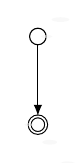
\begin{tikzpicture}[node distance=0.9cm and 0.4cm, every node/.style={scale=.7,transform shape}]
        \node[source] (srcint) {};
        \node[sink,below=of srcint] (sinkint) {};
        \node[mycallout, above = .3cm of srcint, xshift=1cm, callout absolute pointer={(srcint.east)}] {source node};
        \node[mycallout, below = .3cm of sinkint, xshift=1cm, callout absolute pointer={(sinkint.west)}] {sink node};
        \path[line] (srcint) -- (sinkint);
      \end{tikzpicture}
       &
      % gint
      \begin{tikzpicture}[node distance=0.9cm and 0.4cm, every node/.style={scale=.7,transform shape}]
        \mkint{}{int}[]
        \mkgraph{int}{int};
        %       \node[mycallout, above = .3cm of srcint, xshift=1cm, callout absolute pointer={(srcint.east)}] {source node};
        %       \node[mycallout, below = .3cm of sinkint, xshift=-1cm, callout absolute pointer={(sinkint.west)}] {sink node};
      \end{tikzpicture}
       &
      % gseq
      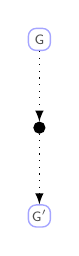
\begin{tikzpicture}[node distance=.9cm and 0.4cm, every node/.style={scale=.7,transform shape}]
        \node[bblock] at (0,0) (g) {$\aG$};
        \node[node, below=of g] (s1) {};
        \node[bblock, below=of s1] (gp) {$\aG'$};
        \path[line,dotted] (g) -- (s1);
        \path[line,dotted] (s1) -- (gp);
      \end{tikzpicture}
       &
      % gpar
      \begin{tikzpicture}[node distance=.4cm and 0.4cm, every node/.style={scale=.7,transform shape}]
        \node[bblock] at (-.7,0) (g) {$\aG$};
        \node[bblock] at (.7,0)  (gp) {$\aG'$};
        \node[node, above=of g] (f) {};
        \node[node, below=of g] (j) {};
        \node[node, above=of gp] (fp) {};
        \node[node, below=of gp] (jp) {};
        \path[line,dotted] (f) -- (g);
        \path[line,dotted] (g) -- (j);
        \path[line,dotted] (fp) -- (gp);
        \path[line,dotted] (gp) -- (jp);
        \mkfork{f,fp}[fork][][#1];
        \mkjoin{j,jp}[join][][#2];
        \mkgraph{fork}{join};
        \node[mycallout, above = .3cm of fork, xshift=-1cm, callout absolute pointer={(fork.west)}] {fork gate};
        \node[mycallout, above = -.9cm of join, xshift=-1cm, callout absolute pointer={(join.west)}] {join gate};
      \end{tikzpicture}
       &
      % gcho
      \begin{tikzpicture}[node distance=.4cm and 0.4cm, every node/.style={scale=.7,transform shape}]
        \node[bblock] at (-.7,0) (g) {$\aG$};
        \node[bblock] at (.7,0)  (gp) {$\aG'$};
        \node[node, above=of g] (f) {};
        \node[node, below=of g] (j) {};
        \node[node, above=of gp] (fp) {};
        \node[node, below=of gp] (jp) {};
        \path[line,dotted] (f) -- (g);
        \path[line,dotted] (g) -- (j);
        \path[line,dotted] (fp) -- (gp);
        \path[line,dotted] (gp) -- (jp);
        \mkbranch{f,fp}[fork][][#3];
        \mkmerge{j,jp}[join][][#4];
        \mkgraph{fork}{join};
        \node[mycallout, above = .3cm of fork, xshift=-1cm, callout absolute pointer={(fork.west)}] {branch gate};
        \node[mycallout, above = -.9cm of join, xshift=-1cm, callout absolute pointer={(join.west)}] {merge gate};
      \end{tikzpicture}
      % &
      % % grec
      % \begin{tikzpicture}[node distance=0.4cm and 0.4cm, every node/.style={scale=.7,transform shape}]
      %   \node[bblock] (g) {$\aG$};
      %   \node[node, above=.5cm of g] (f) {};
      %   \node[node, below=.5cm of g] (j) {};
      %   \path[line,dotted] (f) -- (g);
      %   \path[line,dotted] (g) -- (j);
      %   \mkloop[.5][@]{f}{j}[];
      %   \mkgraph[.4cm]{entryf}{exitj};
      %   \node[mycallout, above = .2cm of entryf, xshift=1.3cm, callout absolute pointer={(entryf.east)}] {loop entry};
      %   \node[mycallout, above = -.7cm of exitj, xshift=-1.3cm, callout absolute pointer={(exitj.west)}] {loop exit};
      % \end{tikzpicture}
      \\
      \text{#6 empty}
       &
      \text{#6 interaction}
       &
      \text{#6 sequential}
       &
      \text{#6 parallel}
       &
      \text{#6 branching}
      % &
      % \text{#6 iteration}
    \end{array}$
}

\newcommandx{\wwwcquote}[1][1=quo:w3c,usedefault=@]{
  \ifempty{#1}{}{\begin{quote}\label{#1}}\renewcommand{\baselinestretch}{-.15}
	 \lq\lq Using the Web Services Choreography specification, a
	 \textcolor{orange}{contract} containing a global definition of the
	 common \textcolor{orange}{ordering} conditions and constraints
	 under which \textcolor{orange}{messages} are exchanged, is
	 produced that describes, from a \textcolor{orange}{global
		viewpoint} [...]  observable behaviour of all the parties
	 involved.
    %
    \textcolor{OliveGreen}{Each party} can then use the global definition to
    \textcolor{OliveGreen}{build and test solutions that conform to it}.
    %
    The global specification is in turn \textcolor{OliveGreen}{realised by combination of} the
    resulting \textcolor{OliveGreen}{local systems} [...]\rq\rq
  \ifempty{#1}{}{\else\end{quote}}
}


%%% Local Variables:
%%% mode: latex
%%% TeX-master: "main"
%%% End:
